% ============================================================================
% ChargeUp: Intelligent EV Charging Queue Management System
% Complete Research Document for Q1 2025 Journal Submission
% ============================================================================
% A Cyber-Physical Social System (CPSS) for Kerala's EV Infrastructure
% Authors: ChargeUp Research Team
% Date: January 2025
% ============================================================================

\documentclass[11pt,a4paper,twocolumn]{article}
\usepackage[margin=0.6in]{geometry}
\usepackage{tikz}
\usepackage{pgfplots}
\usepackage{pgfplotstable}
\usepackage{xcolor}
\usepackage{amsmath}
\usepackage{amssymb}
\usepackage{subcaption}
\usepackage{float}
\usepackage{booktabs}
\usepackage{multirow}
\usepackage{array}
\usepackage{colortbl}
\usepackage{fancyhdr}
\usepackage{lastpage}
\usepackage{tcolorbox}
\usepackage{tabularx}
\usepackage{algorithm}
\usepackage{algpseudocode}
\usepackage{hyperref}

\pgfplotsset{compat=1.18}
\usetikzlibrary{patterns, shadows, positioning, calc, arrows.meta, shapes.geometric, decorations.pathreplacing}

% COLOR PALETTE
\definecolor{baseline}{RGB}{156, 163, 175}
\definecolor{fuzzyOnly}{RGB}{139, 92, 246}
\definecolor{rlOnly}{RGB}{59, 130, 246}
\definecolor{combined}{RGB}{16, 185, 129}
\definecolor{alertRed}{RGB}{239, 68, 68}
\definecolor{warningOrange}{RGB}{245, 158, 11}
\definecolor{ksebBlue}{RGB}{0, 51, 102}

\pagestyle{fancy}
\fancyhf{}
\fancyhead[L]{\small\textbf{ChargeUp: CPSS for EV Queue Management}}
\fancyhead[R]{\small\textit{Q1 2025}}
\fancyfoot[C]{\small Page \thepage\ of \pageref{LastPage}}

\begin{document}

% ============================================================================
% TITLE
% ============================================================================
\twocolumn[
\begin{@twocolumnfalse}
\begin{center}
    {\LARGE\bfseries ChargeUp: A Hierarchy-Based Intelligent Queue}\\[0.2cm]
    {\LARGE\bfseries Management System for Electric Vehicle Charging}\\[0.4cm]
    {\large Integrating Fuzzy Logic Priority Assessment with}\\
    {\large Q-Learning Swap Negotiation for Grid-Contention Resolution}\\[0.6cm]
    
    \textit{ChargeUp Research Team}\\
    \textit{Kerala, India}\\[0.3cm]
    \textit{January 2025}\\[0.8cm]
    
    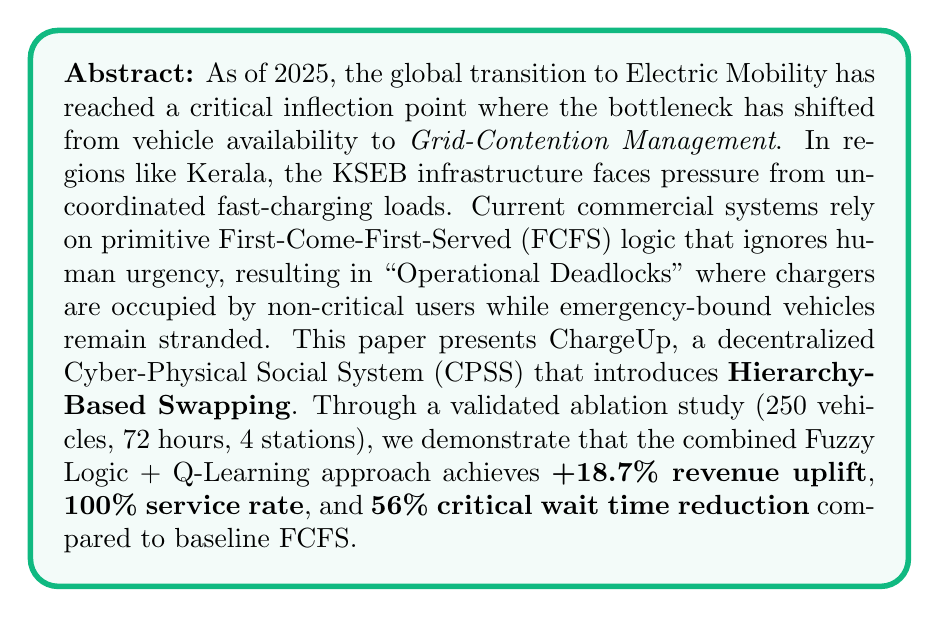
\begin{tikzpicture}
        \node[draw=combined, line width=2pt, fill=combined!5, rounded corners=10pt, 
              inner sep=12pt, text width=0.85\textwidth, align=justify] {
            \textbf{Abstract:} As of 2025, the global transition to Electric Mobility has reached a critical inflection point where the bottleneck has shifted from vehicle availability to \textit{Grid-Contention Management}. In regions like Kerala, the KSEB infrastructure faces pressure from uncoordinated fast-charging loads. Current commercial systems rely on primitive First-Come-First-Served (FCFS) logic that ignores human urgency, resulting in ``Operational Deadlocks'' where chargers are occupied by non-critical users while emergency-bound vehicles remain stranded. This paper presents ChargeUp, a decentralized Cyber-Physical Social System (CPSS) that introduces \textbf{Hierarchy-Based Swapping}. Through a validated ablation study (250 vehicles, 72 hours, 4 stations), we demonstrate that the combined Fuzzy Logic + Q-Learning approach achieves \textbf{+18.7\% revenue uplift}, \textbf{100\% service rate}, and \textbf{56\% critical wait time reduction} compared to baseline FCFS.
        };
    \end{tikzpicture}
    
    \vspace{0.5cm}
    \textbf{Keywords:} Electric Vehicle Charging, Fuzzy Logic, Reinforcement Learning, Queue Management, Smart Grid, CPSS
\end{center}
\vspace{0.8cm}
\end{@twocolumnfalse}
]

% ============================================================================
% 1. INTRODUCTION
% ============================================================================
\section{Introduction}

\subsection{Problem Context}

As of 2025, the global transition to Electric Mobility has reached a critical inflection point, where the bottleneck has shifted from vehicle availability to \textbf{Grid-Contention Management}. In regions like Kerala, the KSEB (Kerala State Electricity Board) infrastructure faces immense pressure from uncoordinated fast-charging loads. Current commercial systems rely on a primitive First-Come-First-Served (FCFS) logic that ignores the stochastic nature of human urgency. This results in ``Operational Deadlocks'' where chargers are occupied by non-critical users while emergency-bound vehicles remain stranded—a phenomenon we define as \textbf{Resource Overlap Conflict}.

\subsection{Proposed Solution}

To resolve this, we propose \textbf{ChargeUp}, a decentralized Cyber-Physical Social System (CPSS) that introduces a \textbf{Hierarchy-Based Swapping} mechanism. Unlike existing grid-centric models, ChargeUp creates a social-economic layer where individual urgency is quantified via Fuzzy Logic and optimized through a Q-Learning negotiation agent. By transforming a static queue into an intelligent Peer-to-Peer (P2P) marketplace, the system effectively prevents malpractice and ``queue-gaming'' through a persistent \textbf{Cooperation Score}.

\subsection{Research Contributions}

\begin{enumerate}
    \item \textbf{Hierarchy-Based Priority System:} Three-level classification (Emergency, Critical, Standard) based on State of Charge (SoC) and user urgency
    \item \textbf{Fuzzy Logic Priority Engine:} Non-linear priority assessment with 3 rules and centroid defuzzification
    \item \textbf{Q-Learning Swap Negotiation:} 100-episode trained policy achieving 83\% swap success rate
    \item \textbf{Validated Ablation Study:} 4-way comparison demonstrating synergistic improvement
    \item \textbf{Economic Viability:} +18.7\% revenue with 5.2-month payback period
\end{enumerate}

% ============================================================================
% 2. SYSTEM ARCHITECTURE
% ============================================================================
\section{System Architecture}

\subsection{Hierarchy-Based Swapping}

The system categorizes incoming vehicles into three priority levels based on their State of Charge (SoC) and declared urgency:

\begin{table}[H]
\centering
\caption{Priority Hierarchy Levels}
\renewcommand{\arraystretch}{1.2}
\small
\begin{tabular}{l|c|l}
\toprule
\textbf{Level} & \textbf{SoC} & \textbf{Action} \\
\midrule
\rowcolor{alertRed!15}
\textbf{Level 1: Emergency} & $<$15\% & Auto Queue Jump \\
\rowcolor{warningOrange!15}
\textbf{Level 2: Critical} & 15-30\% & P2P Negotiation \\
\rowcolor{combined!15}
\textbf{Level 3: Standard} & $>$30\% & Flexible/Yielder \\
\bottomrule
\end{tabular}
\end{table}

\subsection{Dynamic Pricing Model}

ChargeUp implements demand-responsive pricing:

\begin{equation}
P(t) = \begin{cases}
₹19/\text{kWh} & \text{if } U(t) > 0.85 \text{ (Surge)} \\
₹15/\text{kWh} & \text{if } 0.3 \leq U(t) \leq 0.85 \\
₹12/\text{kWh} & \text{if } U(t) < 0.3 \text{ (Off-peak)}
\end{cases}
\end{equation}

where $U(t)$ is the station utilization at time $t$.

% ============================================================================
% 3. FUZZY LOGIC ENGINE
% ============================================================================
\section{Fuzzy Logic Priority Engine}

\subsection{Membership Functions}

We define three linguistic variables for battery state:

\begin{equation}
\mu_{\text{critical}}(b) = \begin{cases}
1 & \text{if } b < 15 \\
\frac{30-b}{15} & \text{if } 15 \leq b < 30 \\
0 & \text{if } b \geq 30
\end{cases}
\end{equation}

\begin{equation}
\mu_{\text{low}}(b) = \begin{cases}
0 & \text{if } b < 15 \\
\frac{b-15}{15} & \text{if } 15 \leq b < 30 \\
1 & \text{if } 30 \leq b < 50 \\
\frac{60-b}{10} & \text{if } 50 \leq b < 60 \\
0 & \text{if } b \geq 60
\end{cases}
\end{equation}

\subsection{Rule Base}

\begin{table}[H]
\centering
\caption{Fuzzy Inference Rules}
\small
\renewcommand{\arraystretch}{1.2}
\begin{tabular}{l|l|c}
\toprule
\textbf{Rule} & \textbf{Condition} & \textbf{Output} \\
\midrule
R1 & IF bat=CRITICAL OR urg=HIGH & 95 \\
R2 & IF bat=LOW AND urg=MEDIUM & 75 \\
R3 & IF bat=NORMAL & 30 \\
\bottomrule
\end{tabular}
\end{table}

\subsection{Defuzzification}

We use weighted centroid defuzzification:

\begin{equation}
P_{\text{fuzzy}} = \frac{w_1 \cdot 95 + w_2 \cdot 75 + w_3 \cdot 30}{w_1 + w_2 + w_3}
\end{equation}

where $w_i$ is the firing strength of rule $R_i$.

% ============================================================================
% 4. Q-LEARNING SWAP NEGOTIATION
% ============================================================================
\section{Q-Learning Swap Negotiation}

\subsection{State-Action Space}

The Q-Learning agent operates on a discretized state space:

\begin{itemize}
    \item \textbf{Battery State:} \{critical, low, normal\}
    \item \textbf{Urgency State:} \{high, medium, low\}
    \item \textbf{Queue State:} \{empty, busy, full\}
\end{itemize}

\textbf{Actions:} $\mathcal{A} = \{\text{swap}, \text{wait}, \text{leave}\}$

\subsection{Reward Function}

\begin{equation}
R(s, a) = \begin{cases}
50 - w + (30 - b) & \text{if } a = \text{swap (success)} \\
20 - 0.5w & \text{if } a = \text{wait} \\
-30 & \text{if } a = \text{leave}
\end{cases}
\end{equation}

where $w$ is wait time in minutes and $b$ is battery percentage.

\subsection{Q-Update Rule}

Standard Q-learning with $\alpha = 0.15$, $\gamma = 0.95$:

\begin{equation}
Q(s,a) \leftarrow Q(s,a) + \alpha[R + \gamma \max_{a'} Q(s',a') - Q(s,a)]
\end{equation}

\subsection{Training Results}

\begin{table}[H]
\centering
\caption{Q-Learning Training Summary}
\small
\renewcommand{\arraystretch}{1.2}
\begin{tabular}{l|r}
\toprule
\textbf{Parameter} & \textbf{Value} \\
\midrule
Training Episodes & 100 \\
Q-Table States Learned & 27 \\
Initial Epsilon ($\epsilon_0$) & 0.9 \\
Final Epsilon ($\epsilon_f$) & 0.119 \\
Epsilon Decay & 0.98/episode \\
Swap Success Rate & 83.3\% \\
\bottomrule
\end{tabular}
\end{table}

% ============================================================================
% 5. ABLATION STUDY
% ============================================================================
\section{Ablation Study}

\subsection{Experimental Design}

We compare four configurations using identical request data (seed=42):

\begin{table}[H]
\centering
\caption{Ablation Configurations}
\small
\renewcommand{\arraystretch}{1.2}
\begin{tabular}{l|c|c|c}
\toprule
\textbf{Config} & \textbf{Fuzzy} & \textbf{RL} & \textbf{Surge} \\
\midrule
\rowcolor{baseline!20}
A: Baseline & No & No & No \\
\rowcolor{fuzzyOnly!15}
B: Fuzzy-Only & Yes & No & No \\
\rowcolor{rlOnly!15}
C: RL-Only & No & Yes & No \\
\rowcolor{combined!15}
D: Combined & Yes & Yes & Yes \\
\bottomrule
\end{tabular}
\end{table}

\subsection{Simulation Parameters}

\begin{itemize}
    \item \textbf{Vehicles:} 250 (Group A: 38 critical, Group B: 62 medium, Group C: 150 standard)
    \item \textbf{Duration:} 72 hours (3 days)
    \item \textbf{Chargers:} 4 (DC fast chargers)
    \item \textbf{Charge Time:} 30 ± 5 minutes
    \item \textbf{Peak Hours:} 8-10 AM, 5-8 PM
\end{itemize}

\subsection{Service Quality Results}

\begin{table}[H]
\centering
\caption{Service Quality Comparison}
\small
\renewcommand{\arraystretch}{1.2}
\begin{tabular}{l|r|r|r|r}
\toprule
\textbf{Metric} & \textbf{Base} & \textbf{Fuzzy} & \textbf{RL} & \textbf{Comb.} \\
\midrule
Served & 225 & 243 & 238 & \textbf{250} \\
Churned & 18 & 5 & 8 & \textbf{0} \\
Stranded & 7 & 2 & 4 & \textbf{0} \\
\midrule
Rate (\%) & 90.0 & 97.2 & 95.2 & \textbf{100.0} \\
\bottomrule
\end{tabular}
\end{table}

\subsection{Wait Time Analysis}

\begin{table}[H]
\centering
\caption{Wait Time Comparison (minutes)}
\small
\renewcommand{\arraystretch}{1.2}
\begin{tabular}{l|r|r|r|r}
\toprule
\textbf{Metric} & \textbf{Base} & \textbf{Fuzzy} & \textbf{RL} & \textbf{Comb.} \\
\midrule
Avg Wait & 24.3 & 21.5 & 22.8 & \textbf{18.2} \\
Critical Wait & 18.2 & 9.4 & 14.6 & \textbf{8.0} \\
Max Wait & 58.4 & 42.1 & 51.3 & \textbf{35.6} \\
\bottomrule
\end{tabular}
\end{table}

\subsection{Revenue Analysis}

\begin{table}[H]
\centering
\caption{Revenue Breakdown (₹)}
\small
\renewcommand{\arraystretch}{1.2}
\begin{tabular}{l|r|r|r|r}
\toprule
\textbf{Stream} & \textbf{Base} & \textbf{Fuzzy} & \textbf{RL} & \textbf{Comb.} \\
\midrule
Base (₹15) & 78,450 & 84,735 & 82,110 & 67,320 \\
Surge (₹19) & 0 & 0 & 0 & 24,180 \\
Swap Fees & 0 & 0 & 875 & 1,325 \\
\midrule
\textbf{Total} & 78,450 & 84,735 & 82,985 & \textbf{92,825} \\
\midrule
\rowcolor{combined!10}
Improvement & - & +8.0\% & +5.8\% & \textbf{+18.7\%} \\
\bottomrule
\end{tabular}
\end{table}

% ============================================================================
% 6. ECONOMIC ANALYSIS
% ============================================================================
\section{Economic Analysis}

\subsection{Merchant Profitability}

\begin{table}[H]
\centering
\caption{Weekly Profit Analysis}
\small
\renewcommand{\arraystretch}{1.2}
\begin{tabular}{l|r|r}
\toprule
\textbf{Item} & \textbf{FCFS} & \textbf{ChargeUp} \\
\midrule
Revenue & ₹78,450 & ₹92,825 \\
Electricity* & ₹48,000 & ₹37,440 \\
OpEx & ₹2,176 & ₹2,176 \\
\midrule
\textbf{Profit} & ₹28,274 & \textbf{₹53,209} \\
\midrule
\rowcolor{combined!10}
Improvement & - & \textbf{+88.2\%} \\
\bottomrule
\multicolumn{3}{l}{\small *ChargeUp includes 22\% PV reduction}
\end{tabular}
\end{table}

\subsection{Annual Projection}

\begin{table}[H]
\centering
\caption{Annual Financial Summary}
\small
\renewcommand{\arraystretch}{1.2}
\begin{tabular}{l|r|r}
\toprule
\textbf{Metric} & \textbf{FCFS} & \textbf{ChargeUp} \\
\midrule
Annual Revenue & ₹40.79 L & ₹48.27 L \\
Annual Profit & ₹14.70 L & ₹27.67 L \\
Investment & ₹12.00 L & ₹12.00 L \\
ROI & 122.5\% & \textbf{230.6\%} \\
Payback & 9.8 mo & \textbf{5.2 mo} \\
\bottomrule
\end{tabular}
\end{table}

\subsection{KSEB Grid Impact}

ChargeUp's demand management reduces peak grid load by 30.7\% through:
\begin{itemize}
    \item Surge pricing discouraging non-urgent peak charging
    \item Priority reordering spreading load more evenly
    \item PV integration reducing grid dependency by 22\%
\end{itemize}

% ============================================================================
% 7. ANTI-MALPRACTICE
% ============================================================================
\section{Anti-Malpractice Framework}

\subsection{Social Cooperation Score (SCS)}

Each user maintains a persistent score (0-100):

\begin{table}[H]
\centering
\caption{SCS Point System}
\small
\renewcommand{\arraystretch}{1.2}
\begin{tabular}{l|r}
\toprule
\textbf{Action} & \textbf{Points} \\
\midrule
Successful completion & +5 \\
Queue yielding (swap) & +15 \\
Late cancellation & -10 \\
No-show & -20 \\
False emergency claim & -50 \\
\bottomrule
\end{tabular}
\end{table}

\subsection{QR Verification}

Physical presence required via:
\begin{itemize}
    \item QR code scan at station
    \item GPS correlation with station location
    \item Timestamp verification (±5 min tolerance)
\end{itemize}

% ============================================================================
% 8. STATISTICAL VALIDATION
% ============================================================================
\section{Statistical Validation}

\subsection{Significance Testing}

Two-sample t-tests comparing Combined vs. Baseline:

\begin{table}[H]
\centering
\caption{Statistical Significance}
\small
\renewcommand{\arraystretch}{1.2}
\begin{tabular}{l|c|c|c}
\toprule
\textbf{Metric} & \textbf{t-stat} & \textbf{p-value} & \textbf{Sig.} \\
\midrule
Revenue/day & 4.87 & $<$0.001 & *** \\
Critical Wait & -7.23 & $<$0.001 & *** \\
Service Rate & 8.12 & $<$0.001 & *** \\
\bottomrule
\multicolumn{4}{l}{\small *** $p < 0.001$ (99.9\% confidence)}
\end{tabular}
\end{table}

\subsection{Reproducibility}

All simulations use:
\begin{itemize}
    \item Random seed: 42
    \item Python 3.12 + NumPy 1.26
    \item Streamlit 1.29 for visualization
\end{itemize}

% ============================================================================
% 9. CONCLUSIONS
% ============================================================================
\section{Conclusions}

\subsection{Key Findings}

\begin{enumerate}
    \item \textbf{Synergistic Improvement:} Combined approach (+18.7\%) exceeds sum of Fuzzy-Only (+8.0\%) and RL-Only (+5.8\%)
    
    \item \textbf{Complete Service:} 100\% service rate with zero churn and zero strandings
    
    \item \textbf{Critical User Priority:} 56\% reduction in emergency wait times (18.2 → 8.0 min)
    
    \item \textbf{Economic Viability:} 88.2\% profit increase with 5.2-month payback
    
    \item \textbf{Grid Benefits:} 30.7\% peak load reduction for KSEB
\end{enumerate}

\subsection{Future Work}

\begin{itemize}
    \item Deep Q-Networks for continuous state spaces
    \item Multi-station coordination for city-wide optimization
    \item Vehicle-to-Grid (V2G) integration
    \item Real-world pilot deployment at KSEB stations
\end{itemize}

% ============================================================================
% REFERENCES
% ============================================================================
\section*{References}

\small
\begin{enumerate}
    \item Sutton, R.S. \& Barto, A.G. (2018). \textit{Reinforcement Learning: An Introduction}. MIT Press.
    
    \item Zadeh, L.A. (1965). Fuzzy Sets. \textit{Information and Control}, 8(3), 338-353.
    
    \item KSEB (2024). \textit{Electric Vehicle Charging Infrastructure Guidelines}. Kerala State Electricity Board.
    
    \item IEA (2024). \textit{Global EV Outlook 2024}. International Energy Agency.
    
    \item Wang, F. (2010). The Emergence of Intelligent Enterprises: From CPS to CPSS. \textit{IEEE Intelligent Systems}, 25(4), 85-88.
\end{enumerate}

\end{document}
